\documentclass[ignorenonframetext,]{beamer}

\setbeamertemplate{caption}[numbered]
\setbeamertemplate{caption label separator}{: }
\setbeamercolor{caption name}{fg=normal text.fg}

\beamertemplatenavigationsymbolsempty
\usepackage{lmodern}
\usepackage{amssymb,amsmath}
\usepackage{ifxetex,ifluatex}
\usepackage{fixltx2e} % provides \textsubscript
\ifnum 0\ifxetex 1\fi\ifluatex 1\fi=0 % if pdftex
  \usepackage[T1]{fontenc}
  \usepackage[utf8]{inputenc}
\else % if luatex or xelatex
  \ifxetex
    \usepackage{mathspec}
  \else
    \usepackage{fontspec}
  \fi
  \defaultfontfeatures{Ligatures=TeX,Scale=MatchLowercase}
\fi

% Start adding some content
\usepackage{graphicx}
\usepackage{color}
\usepackage{beamerthemebars}
\usepackage{multicol}
\usepackage{multirow}
\usepackage{hyperref}


\usetheme{Frankfurt}
%%redefined colors for beamer
%\definecolor{beamer@UIUCblue}{RGB}{0,60,125}
%\definecolor{beamer@UIUCorange}{RGB}{244,127,36}
%% taken from
%% http://identitystandards.illinois.edu/graphicstandardsmanual/generalguidelines/colors.html
%
%\definecolor{beamer@UIUCgray}{RGB}{210,210,210}
%\definecolor{beamer@UIUCgray2}{RGB}{244,244,244}
%
%\setbeamercolor{frametitle}{fg=beamer@UIUCblue,bg=beamer@UIUCgray}
%\setbeamercolor{normal text}{fg=black}
%\setbeamercolor{title}{fg=beamer@UIUCblue,bg=beamer@UIUCorange}
%\setbeamercolor{item projected}{fg=white,bg=beamer@UIUCorange}
%
%% Boxes
%\setbeamercolor{block title}{fg=beamer@UIUCblue,bg=beamer@UIUCorange}
%\setbeamercolor{block body}{fg=blue,bg=beamer@UIUCblue!80}
%\setbeamercolor{title in head/foot}{fg=beamer@UIUCblue,bg=beamer@UIUCgray}
%\setbeamercolor{author in head/foot}{fg=white,bg=beamer@UIUCblue}
%\setbeamercolor{institute in head/foot}{fg=white,bg=beamer@UIUCorange}
%\setbeamercolor{date in head/foot}{fg=white,bg=beamer@UIUCorange}
%\setbeamercolor{section in head/foot}{fg=white,bg=beamer@UIUCblue}
%\setbeamercolor{subsection in head/foot}{fg=white,bg=beamer@UIUCorange}
%
%
%\hypersetup{colorlinks=true,urlcolor=beamer@UIUCblue,linkcolor=beamer@UIUCblue,% link color controls section, subsection, and title
%citecolor = beamer@UIUCorange,
%anchorcolor = beamer@UIUCorange}
%
%%override title link color
%\addtobeamertemplate{headline}{\hypersetup{linkcolor=.}}{}
%\addtobeamertemplate{footline}{\hypersetup{linkcolor=.}}{}
%
%% Setup blocks
%\setbeamercolor{block title}{fg = white, bg = beamer@UIUCblue}
%\setbeamercolor{block body}{fg=black,bg=beamer@UIUCgray2}
%
%\setbeamercolor{block title alerted}{fg = white, bg = beamer@UIUCorange}
%\setbeamercolor{block body alerted}{fg=black,bg=beamer@UIUCgray2}
%
%\setbeamercolor{block title example}{fg = beamer@UIUCblue, bg = beamer@UIUCgray}
%\setbeamercolor{block body example}{fg=black,bg=beamer@UIUCgray2}

% use upquote if available, for straight quotes in verbatim environments
\IfFileExists{upquote.sty}{\usepackage{upquote}}{}
% use microtype if available
\IfFileExists{microtype.sty}{%
\usepackage{microtype}
\UseMicrotypeSet[protrusion]{basicmath} % disable protrusion for tt fonts
}{}
\newif\ifbibliography
\usepackage{graphicx,grffile}
\makeatletter
\def\maxwidth{\ifdim\Gin@nat@width>\linewidth\linewidth\else\Gin@nat@width\fi}
\def\maxheight{\ifdim\Gin@nat@height>\textheight0.8\textheight\else\Gin@nat@height\fi}
\makeatother
% Scale images if necessary, so that they will not overflow the page
% margins by default, and it is still possible to overwrite the defaults
% using explicit options in \includegraphics[width, height, ...]{}
\setkeys{Gin}{width=\maxwidth,height=\maxheight,keepaspectratio}

% Prevent slide breaks in the middle of a paragraph:
\widowpenalties 1 10000
\raggedbottom

\AtBeginSection[]
{
  \ifbibliography
  \else
    \let\insertsectionnumber\relax
    \let\sectionname\relax
    \begin{frame}
      \frametitle{On the Agenda}
      \begin{multicols}{2}
      \tableofcontents[currentsection]
      \end{multicols}
    \end{frame}
  \fi
}

\setlength{\parindent}{0pt}
\setlength{\parskip}{6pt plus 2pt minus 1pt}
\setlength{\emergencystretch}{3em}  % prevent overfull lines
\providecommand{\tightlist}{%
  \setlength{\itemsep}{0pt}\setlength{\parskip}{0pt}}
\setcounter{secnumdepth}{0}
\usepackage{amsmath, bbm, graphicx,multirow}
\usepackage{booktabs}
\usepackage{caption}
\usepackage{longtable}
\usepackage{array}
\usepackage{blkarray}
\usepackage{multirow}
\usepackage{wrapfig}
\usepackage{float}
\usepackage{colortbl}
\usepackage{pdflscape}
\usepackage{tabu}
\usepackage{threeparttable}
\usepackage{threeparttablex}
\usepackage[normalem]{ulem}
\usepackage{makecell}
\usepackage{xcolor}
\newcolumntype{Z}{>{\setbox0=\hbox\bgroup}c<{\egroup}@{\hspace*{-\tabcolsep}}}
\newcommand{\indep}{\rotatebox[origin=c]{90}{$\models$}}


\author[
Xuelong Wang and Jie Yang
]{Xuelong Wang and Jie Yang}
\institute[
UIC
]{
Department of Mathematics, Computer Science, and Statistics \\
University of Illinois at Chicago
}
\date[
09/09/2019
]{
September 09, 2019
}

% Option to fake out the raw_tex plugin and, thus, enabling the embedding of
% markdown within a column scheme.
% See:
% (1) https://groups.google.com/forum/#!msg/pandoc-discuss/vcy7v9Uk95U/LDgWJTHTRR4J
% (2) http://stackoverflow.com/questions/15142134/slides-with-columns-in-pandoc
\def\begincols{\begin{columns}}
\def\endcols{\end{columns}}

\begin{document}

% Necessary due to the ignorenonframetext requirement
% See: http://tex.stackexchange.com/questions/181032/ignorenonframetext-option-breaks-frame-background-color-option
\mode<all>{
\title[
Representative approach
]{
%\begin{columns}
%\column{.25\textwidth}
%\hspace{.2in}
%\vspace{.1in}
%\includegraphics{ilogo.pdf}
%\column{.85\textwidth}
Representative approach for big data dimension reduction with binary
responses
%\end{columns}
}
}
\mode*

\frame{\titlepage}

\begin{frame}
\tableofcontents[hideallsubsections]
\end{frame}

\section{Motivation}\label{motivation}

\subsection{Motivation}\label{motivation-1}

\begin{frame}{Motivation of dimension reduction}

\begin{block}{Issues of high dimensional data (p is large)}

\begin{itemize}
\tightlist
\item
  Curse of dimensionality (e.g.~data points become sparse)\\
\item
  Model overfitting
\end{itemize}

\end{block}

\begin{block}{Two approaches}

\begin{enumerate}
\def\labelenumi{\arabic{enumi}.}
\tightlist
\item
  Variable selection

  \begin{itemize}
  \tightlist
  \item
    Forward/Backward selection, Shrinkage method (Lasso), etc.
  \end{itemize}
\item
  \textbf{Dimension reduction} (Variable Projection)

  \begin{itemize}
  \tightlist
  \item
    Principle component analysis
  \item
    Sufficient dimension reduction
  \end{itemize}
\end{enumerate}

\end{block}

\end{frame}

\begin{frame}{An example: Breast cancer data}

\begin{columns}
\begin{column}{0.5\textwidth}
   \begin{block}{Data}
    \begin{itemize}
    \item X: 30 Dependent variables are computed from a digitized image of a breast mass
    \item Y: Diagnosis results\\ 
    (1 = malignant, 0 = benign)
    \end{itemize}
   \end{block}
\end{column}
\begin{column}{0.5\textwidth}  %%<--- here
    \begin{block}{A Sample picture}
    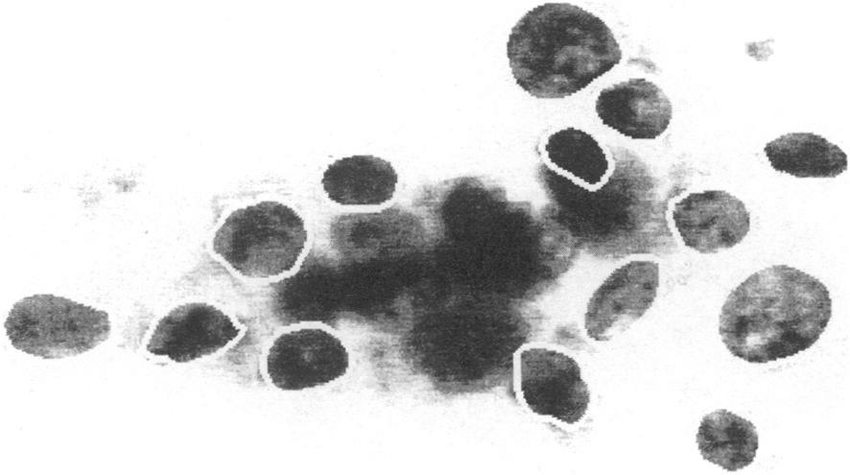
\includegraphics{./pic/breast_cancer.png}
    \end{block}
\end{column}
\end{columns}

\begin{block}{Goal}

Classification: Diagnose breast cancer from image-processed variables

\end{block}

\end{frame}

\begin{frame}{An example: Breast cancer data}

\begin{center}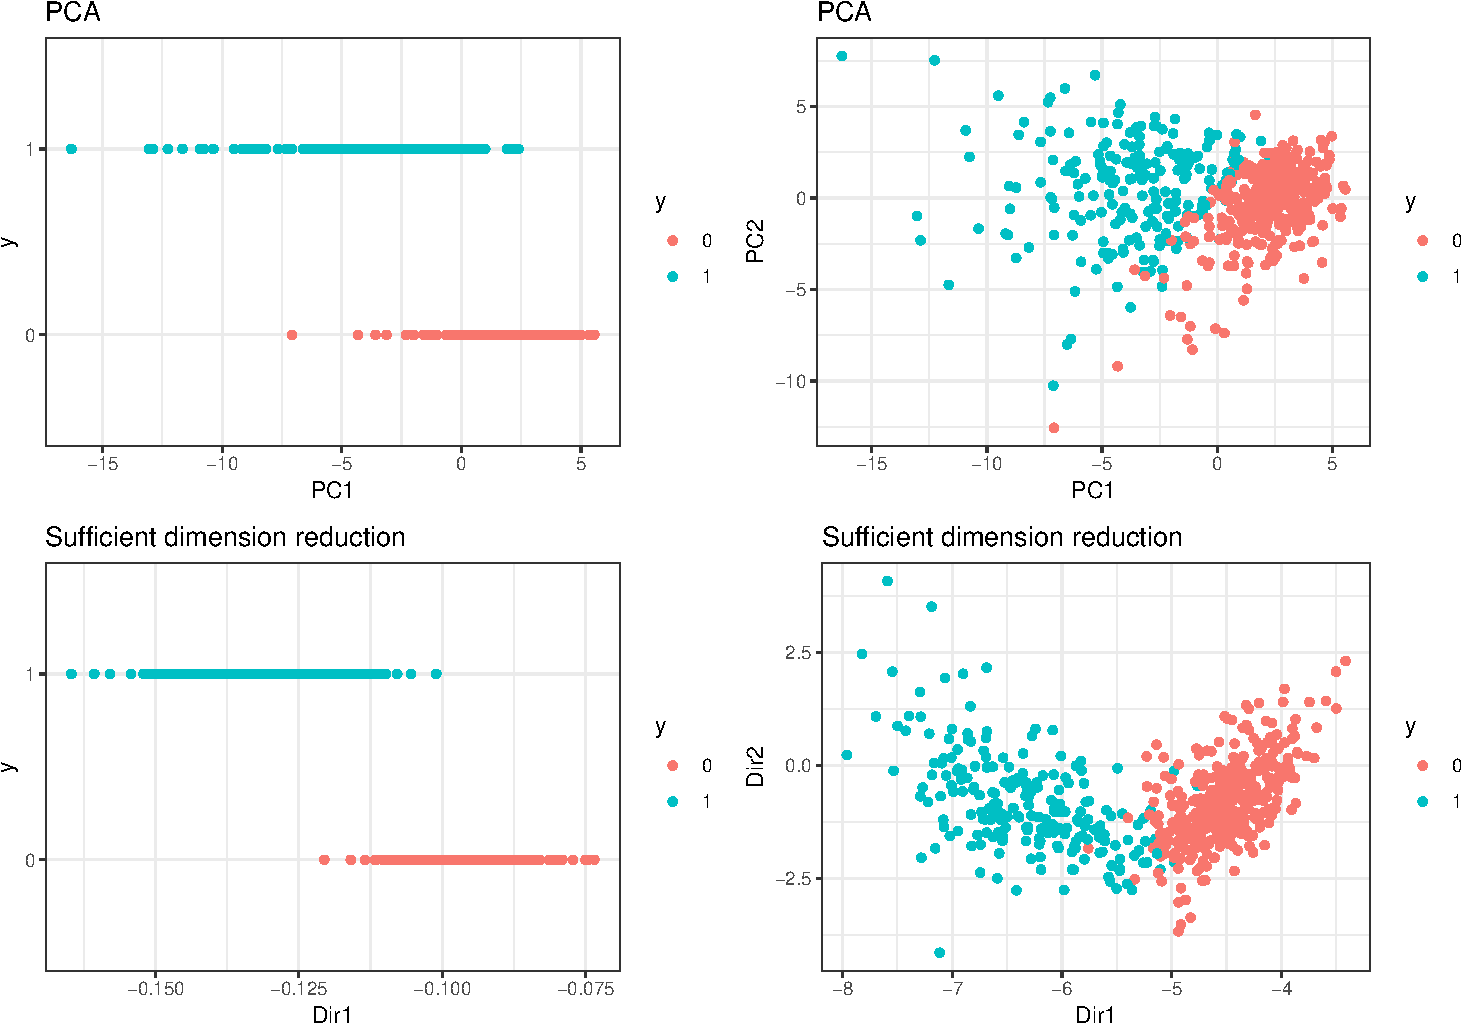
\includegraphics{SDR_reps_slides_final_merck_files/figure-beamer/unnamed-chunk-2-1} \end{center}

\end{frame}

\section{Background and Issue}\label{background-and-issue}

\subsection{SDR}\label{sdr}

\begin{frame}{Span and basis}

Given d independent vectors
\(B = (\mathbf{b}_1, \dots, \mathbf{b}_d), ~~\mathbf{b}_i \in \mathbb{R}^p\),
\[
\text{Subspace }V = \mathcal{L}(\mathbf{b}_1, \dots, \mathbf{b}_d) = \{\sum_{i = 1}^k\lambda_i\mathbf{b}_i, \lambda_i\in \mathbb{R}\}
\]

\begin{itemize}
\tightlist
\item
  \(V = span(\mathbf{b}_1, \dots, \mathbf{b}_d)\), \(V\) is spanned by
  B,\\
\item
  \(B = (\mathbf{b}_1, \dots, \mathbf{b}_d)\) is a basis of \(V\)\\

  \begin{columns}
  \begin{column}{0.6\textwidth}
     \begin{block}{Basis is not unique}
  \[
    Span
  \begin{blockarray}{cc}
  b_1 & b_2  \\
  \begin{block}{(cc)}
    1 & 0 \\
    0 & 1 \\
  \end{block}
  \end{blockarray} \Leftrightarrow 
   Span
  \begin{blockarray}{cc}
  b'_1 & b'_2  \\
  \begin{block}{(cc)}
    1 & 1 \\
    1 & -1 \\
  \end{block}
  \end{blockarray}
    \]
     \end{block}
  \end{column}
  \begin{column}{0.4\textwidth}  %%<--- here
  \begin{block}{Example}
  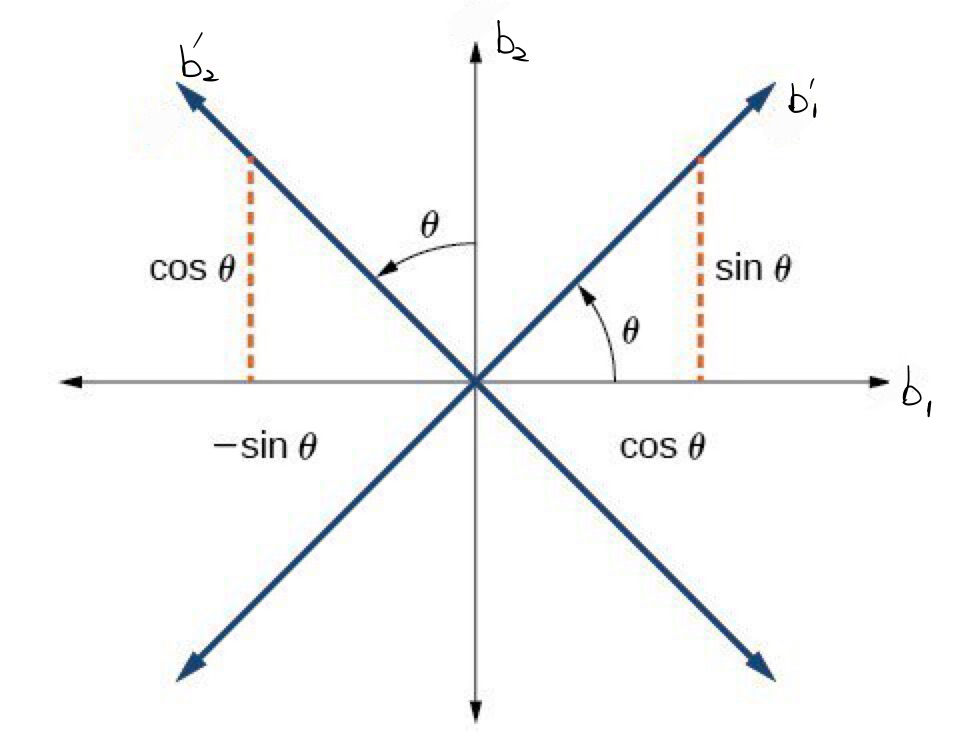
\includegraphics[height=3cm]{./pic/axes-rotation.jpg}
  \end{block}
  \end{column}
  \end{columns}
\end{itemize}

\end{frame}

\begin{frame}{Sufficient dimension reduction}

\begin{block}{Fundamental assumption}

Let random vector \(X \in \mathbb{R}^{p \times 1}\),
\(Y \in \mathbb{R}\),
\(B = (\mathbf{b}_1, \dots,\mathbf{b}_d) \in \mathbb{R}^{p\times d}\),
where \(d << p\) and \(A \in \mathbb{R}^{d\times d}\) is a non-singular
matrix. \[
Y|X \stackrel{d}{=} Y|B^T X
\]

\[
  Y \indep X|B^TX \Rightarrow Y \indep X|(BA)^TX, 
\] So \(B\) is not identifiable, but \(span(B)\) is identifiable.

\end{block}

\end{frame}

\begin{frame}{Sufficient dimension reduction}

\begin{block}{Dimension-reduction subspace (DRS)}

\[
  Y \indep X|P_SX,~~ P_\mathcal{S} = B(B^TB)^{-1}B^T
\] \(\mathcal{S}\) is called the dimension-reduction subspace.

However,\(\mathcal{S}\) is not unique. Actually if
\(\mathcal{S} \subset \mathcal{S}_1\), then \(\mathcal{S}_1\) is also a
dimension-reduction space.

\end{block}

\begin{block}{Target: Central Subspace}

\[
S_{Y|X} = \cap S_{DRS}
\] Under mild conditions, \(S_{Y|X}\) is unique and a DRS subspace
itself (Cook, 1996).

\end{block}

\end{frame}

\begin{frame}{Take home message}

\begin{itemize}
\tightlist
\item
  No model assumption between X and Y\\
\item
  Target is a basis of the central subspace not specific values of
  coefficients
\item
  A basis of subspace is \(B = (\mathbf{b}_1, \dots, \mathbf{b}_d)\)
\end{itemize}

\end{frame}

\subsection{Estimating the central
subspace}\label{estimating-the-central-subspace}

\begin{frame}{Estimating the central subspace}

\begin{block}{Principle component analysis (PCA)}

\begin{enumerate}
\def\labelenumi{\arabic{enumi}.}
\tightlist
\item
  \(M = {Var}(X)\)\\
\item
  Find the eigenvalues of \(M\) and arrange them in descending order
  \(\lambda_1 \geq \dots, \lambda_p\) and their corresponding
  eigenvectors \((u_1, \dots, u_p)\)\\
\item
  Select first several eigenvectors based on the total variation\\
\item
  \((\hat u_1, \dots, \hat u_d) = (\hat{\mathbf{b}}_1, \dots, \hat{\mathbf{b}}_d)\)
\end{enumerate}

\end{block}

\end{frame}

\begin{frame}{Estimating the central subspace (cont.)}

\begin{block}{Sliced Inverse Regression (SIR) (Li 1991)}

\begin{enumerate}
\def\labelenumi{\arabic{enumi}.}
\tightlist
\item
  \(Z = \Sigma_X^{-1/2}(X - E(X))\)
\item
  \(M_{SIR} := \Sigma_X^{1/2}Var(E(Z|Y))\)
\item
  Find the eigenvalues and eigenvectors of \(M_{SIR}\)
\end{enumerate}

\end{block}

\begin{block}{Sliced Average Variance Estimation (SAVE) (Cook et al.
1991)}

\begin{enumerate}
\def\labelenumi{\arabic{enumi}.}
\tightlist
\item
  \(Z = \Sigma_X^{-1/2}(X - E(X))\)
\item
  \(Var(Z|Y)\) is the conditional variance of X given Y
\item
  \(M_{SAVE} := f(Var(Z|Y))\)
\item
  Find the eigenvalues and eigenvectors of \(M_{SAVE}\)
\end{enumerate}

\end{block}

\end{frame}

\begin{frame}{How to estimate the \(E(Z|Y)\), \(Var(Z|Y)\)?}

\begin{enumerate}
\def\labelenumi{\arabic{enumi}.}
\tightlist
\item
  Sort the data based on the response \[
    Y_1 \dots, Y_n \Rightarrow Y^{(1)},\dots,Y^{(n)} 
  \]
\item
  Split data into H slices based on sorted \(Y^{(i)}\)
\item
  Within the slice h, calculate the \(\hat{E}(Z|Y)\),
  \(\hat{Var}(Z|Y)\),
  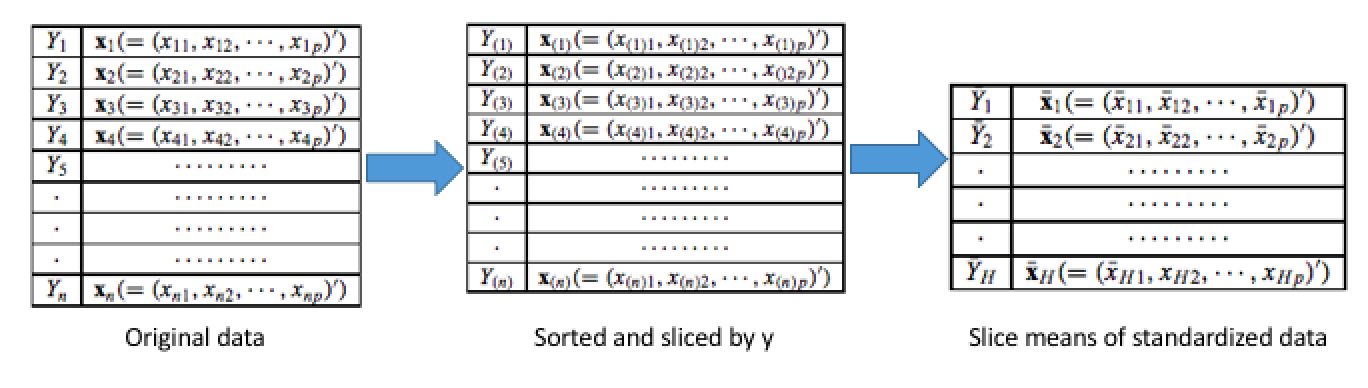
\includegraphics[width=4.16667in]{./pic/slice method.png}
\end{enumerate}

\end{frame}

\begin{frame}{Issue with Binary response}

\begin{itemize}
\item
  A binary response only has two levels, e.g. \(0,1\).
\item
  Only two slices are available after slicing
\item
  SIR can only find one direction
\end{itemize}

\end{frame}

\section{Existing solution}\label{existing-solution}

\subsection{Variance matrix}\label{variance-matrix}

\begin{frame}{Using conditional variance (Cook. 1999)}

\begin{block}{Main Idea}

\(\Delta = \Sigma_{X|Y = 1} - \Sigma_{X|Y = 0}\) could contain all the
information of the central space

\end{block}

\begin{block}{Not full rank}

There are cases that \(\hat \Delta\) is not full rank or even is 0
matrix

\end{block}

\end{frame}

\subsection{PRE}\label{pre}

\begin{frame}{Probability Enhanced (PRE) method (Shin et al. 2014)}

\begin{block}{Main idea}

\begin{itemize}
\tightlist
\item
  \(S_{Y|X} = S_{G(X)|X}\), \(G(x) = \mathcal{P}(Y = 1|X = x)\) is the
  conditional probability
\item
  \(Y \Rightarrow G(X) \in [0,1]\)
\item
  Weighted Support Vector Machine(WSVM) to estimate the \(\hat{G}(X)\)
\end{itemize}

\end{block}

\begin{block}{Computational time}

\begin{itemize}
\tightlist
\item
  SVM method is sensitive to the number of observation N
\item
  Tunning parameters
\end{itemize}

\end{block}

\end{frame}

\section{Our approach}\label{our-approach}

\subsection{Representative}\label{representative}

\begin{frame}{Representative approach}

\begin{block}{Representative}

A Representative is a summary statistic of data points within a cluster:
For \((X_i, Y_i), i \in I_k\) and \(n_k\) is sample size of \(I_k\) \[
  \bar{X}_k = R(X_{1}, \dots, X_{n_k}) = \frac{\sum_i X_i}{n_k},~~ \bar{Y}_k = R(Y_{1}, \dots, Y_{n_k}) = \frac{\sum_i Y_i}{n_k},
\] where \(R\) is the summarizing function.

\end{block}

\begin{block}{Steps}

\begin{enumerate}
\def\labelenumi{\arabic{enumi}.}
\tightlist
\item
  Cluster \((X_1, \dots,X_N)\) into k groups \(I_1, \dots, I_k\),
  e.g.k-means
\item
  Calculate the representatives for each cluster \(I_k\)
\item
  Apply dimension reduction methods on the k representatives
\end{enumerate}

\end{block}

\end{frame}

\begin{frame}{How it works}

\begin{block}{Main idea}

Y and \(G(X)\) have identical central space: \(S_{Y|X} = S_{G(X)|X}\)

\begin{center}
$Y = f(\mathbf{b}_1^TX, \dots, \mathbf{b}_d^TX,\epsilon)$
$\Rightarrow$
$\mathcal{P}(Y = 1 |X) = G(\mathbf{b}_1^TX, \dots, \mathbf{b}_d^TX)$
\end{center}

\end{block}

\begin{block}{For the Representative}

\begin{center}
$\bar{Y}_k = \hat{\mathcal{P}}(Y = 1|X_i, i\in I_k) \approx  G(\bar{X}_k) = G(\mathbf{b}_1^T\bar{X}_k, \dots, \mathbf{b}_d^T\bar{X}_k)$
\end{center}

\end{block}

\end{frame}

\begin{frame}{Aysmptotic property}

Let \(K\) be the total number of clusters, \(n_k\) be the total
observations within cluster k, \(v_k\) be the cluster's volume.

\begin{block}{Cluster with fixed volume}
In this case, K and $v_k$ are fixed, $n_k \to \infty$ as $N \to \infty$
\[
\bar{Y}_k - G(\bar{\mathbf X}_k) \stackrel{P}{\longrightarrow} \mu_g - G(\boldsymbol{\mu}_k)  \neq 0
\]
\end{block}

\begin{block}{Cluster with shrinking volume}
In this case, $K \to \infty,~v_k \to 0, n_k \to \infty $ as $N \to \infty$
\[
E([\bar{Y}_k - G(\bar{\mathbf X}_k)]^2) = O(N^{-\delta(r)})
\]
\end{block}

\begin{itemize}
\tightlist
\item
  \(K = O(N^\frac{p}{4+p})\)
\end{itemize}

\end{frame}

\begin{frame}{Additional value: Big data solution (N is large)}

\begin{block}{Clustering step}

Clustering step reduced the sample size from \(N\) to \(K\).

\begin{itemize}
\tightlist
\item
  \((Y_1,X_1) \dots (Y_N,X_N) \to (\bar{Y}_1,\bar{X}_1) \dots (\bar{Y}_k,\bar{X}_K)\)
\end{itemize}

\end{block}

\begin{block}{Parallel Algorithm for SIR and SAVE}

\begin{enumerate}
\def\labelenumi{\arabic{enumi}.}
\tightlist
\item
  Split the sliced data into b blocks, \(X_1, \dots X_B\)\\
\item
  Load each block \(X_b\) and calculate the statistics for each block
  such as \(\bar{X}_b, X^T_{b}X_{b}\)\\
\item
  Summary the statistics across the blocks to get the candidate matrix
  \(M_{SIR}, M_{SAVE}\)
\end{enumerate}

\end{block}

\end{frame}

\section{Simulation Study}\label{simulation-study}

\subsection{}\label{section}

\begin{frame}{Simulation setup}

\begin{block}{Data generation model: logit model}
\[
    \log\left(\frac{\mathcal{P}(Y=1|X)}{\mathcal{P}(Y=0|X)}\right) = (\mathbf{b}_1^TX)^2 \cdot sin(\mathbf{b}_2^TX) \cdot exp(\mathbf{b}_3^TX)
\]
\begin{itemize}
\item $X \in \mathbb{R}^6$   
\item $\mathbf{b}_i = \mathbf{e}_i = (0, \dots, 1, \dots,0) \in \mathbb{R}^6$  
\item $S_{Y|X} = Span(\mathbf{e}_1, \mathbf{e}_2, \mathbf{e}_3)$   
\item $n = \{10^3, 10^4, 10^5,10^6\}$    
\end{itemize}
\end{block}

\end{frame}

\begin{frame}{How to evaluate estimated central subspace}

\begin{block}{The number of direction}
\begin{itemize}
\item Hypothesis Test: test if a eigenvalue is significant different than 0
\end{itemize}
\end{block}

\begin{columns}
\begin{column}{0.5\textwidth}
   \begin{block}{Frobenius Distance}
    \[
      F = \Vert P_B - P_A\Vert_F
    \]
    \begin{itemize}
    \item $P_A = A(A^TA)^{-1}A$
    \item $\Vert A\Vert_F = \sqrt{\sum_i\sum_j a^2_{ij}}$
    \item small value is better 
    \item 0 means $Span(A) = Span(B)$
    \end{itemize}
    
   \end{block}
\end{column}
\begin{column}{0.5\textwidth}  %%<--- here
    \begin{block}{Trace correlation (R)}
    \[
    R = 1 - \frac{1}{k}\sum_{i=1}^k\rho_i^2
    \]
    \begin{itemize}
      \item $\rho_i^2$ is the eigenvalues of $B^TAA^TB$
      \item small value is better
      \item 0 means $Span(A) \subseteq Span(B)$
    \end{itemize}
    \end{block}
\end{column}
\end{columns}

\end{frame}

\begin{frame}{Result table}

\begin{table}[]
\centering
\caption{Simulation result of table}
\resizebox{\textwidth}{!}{%
\begin{tabular}{|c|c|ZZZZ|ZZZZ|}
\hline
\multicolumn{2}{|c|}{\multirow{2}{*}{}}              & \multicolumn{4}{c|}{ Method A } & \multicolumn{4}{c|}{ Method B}                \\ \cline{3-10} 
\multicolumn{2}{|c|}{}                               & \multicolumn{8}{c|}{log n}                                                      \\ \hline
                          & $H_0$ vs $H_1$       & 3      & 4      & 5      & 6      & 3    & 4    & 5             & 6             \\ \hline
\multirow{3}{*}{Power}    & 0D vs \textgreater{}= 1D & 0.9    & 1      & 1      & 1      & 0    & 0.05 & \color{blue}\textbf{1}    & \color{blue}\textbf{1}    \\
                          & 1D vs \textgreater{}= 2D & 0.08   & 0.52   & 0.52   & 0.5    & 0    & 0    & \color{blue}\textbf{1}    & \color{blue}\textbf{1}    \\
                          & 2D vs \textgreater{}= 3D & 0      & 0.05   & 0.06   & 0.06   & 0    & 0    & 0.05          & \color{blue}\textbf{1}    \\ \hline
\multirow{3}{*}{Type-I error}   & 3D vs \textgreater{}= 4D & 0      & 0      & 0      & 0.01   & 0    & 0    & 0             & 0.14          \\
                          & 4D vs \textgreater{}= 5D & 0      & 0      & 0      & 0      & 0    & 0    & 0             & 0.03             \\
                          & 5D vs \textgreater{}= 6D & 0      & 0      & 0      & 0      & 0    & 0    & 0             & 0.02             \\ \hline
\multirow{2}{*}{Distance} & Frobenius                        & 1.47   & 1.2    & 1.21   & 1.21   & NA & 1.44 & \color{blue}\textbf{1.00} & \color{blue}\textbf{0.39} \\
                          & Trace                        & 0.06   & 0.01   & 0.01   & 0.01   & NA & 0.02  & \color{blue}\textbf{0.01} & \color{blue}\textbf{0.04}    \\ \hline
\end{tabular}%
}
\end{table}

\end{frame}

\begin{frame}{Simulation result of SAVE}

\begin{table}[]
\centering
\caption{Simulation result of SAVE  \newline 
         Significant level 0.05\newline 
         directions of central subsapce $d =3$}\resizebox{\textwidth}{!}{%
\begin{tabular}{|c|c|cccc|cccc|}
\hline
\multicolumn{2}{|c|}{\multirow{2}{*}{}}              & \multicolumn{4}{c|}{Original SAVE} & \multicolumn{4}{c|}{Proposed SAVE}                \\ \cline{3-10} 
\multicolumn{2}{|c|}{}                               & \multicolumn{8}{c|}{log n}                                                      \\ \hline
                          & $H_0$ vs $H_1$       & 3      & 4      & 5      & 6      & 3    & 4    & 5             & 6             \\ \hline
\multirow{3}{*}{Power}    & 0D vs \textgreater{}= 1D & 0.9    & 1      & 1      & 1      & 0    & 0.05 & \color{blue}\textbf{1}    & \color{blue}\textbf{1}    \\
                          & 1D vs \textgreater{}= 2D & 0.08   & 0.52   & 0.52   & 0.5    & 0    & 0    & \color{blue}\textbf{1}    & \color{blue}\textbf{1}    \\
                          & 2D vs \textgreater{}= 3D & 0      & 0.05   & 0.06   & 0.06   & 0    & 0    & 0.05          & \color{blue}\textbf{1}    \\ \hline
\end{tabular}%
}
\end{table}

\end{frame}

\begin{frame}{Simulation result of SAVE}

\begin{table}[]
\centering
\caption{Simulation result of SAVE  \newline 
         Significant level 0.05\newline 
         directions of central subsapce $d =3$}\resizebox{\textwidth}{!}{%
\begin{tabular}{|c|c|cccc|cccc|}
\hline
\multicolumn{2}{|c|}{\multirow{2}{*}{}}              & \multicolumn{4}{c|}{Original SAVE} & \multicolumn{4}{c|}{Proposed SAVE}                \\ \cline{3-10} 
\multicolumn{2}{|c|}{}                               & \multicolumn{8}{c|}{log n}                                                      \\ \hline
                          & $H_0$ vs $H_1$       & 3      & 4      & 5      & 6      & 3    & 4    & 5             & 6             \\ \hline
\multirow{3}{*}{Power}    & 0D vs \textgreater{}= 1D & 0.9    & 1      & 1      & 1      & 0    & 0.05 & \color{blue}\textbf{1}    & \color{blue}\textbf{1}    \\
                          & 1D vs \textgreater{}= 2D & 0.08   & 0.52   & 0.52   & 0.5    & 0    & 0    & \color{blue}\textbf{1}    & \color{blue}\textbf{1}    \\
                          & 2D vs \textgreater{}= 3D & 0      & 0.05   & 0.06   & 0.06   & 0    & 0    & 0.05          & \color{blue}\textbf{1}    \\ \hline
\multirow{3}{*}{Type-I error}   & 3D vs \textgreater{}= 4D & 0      & 0      & 0      & 0.01   & 0    & 0    & 0             & 0.14          \\
                          & 4D vs \textgreater{}= 5D & 0      & 0      & 0      & 0      & 0    & 0    & 0             & 0.03             \\
                          & 5D vs \textgreater{}= 6D & 0      & 0      & 0      & 0      & 0    & 0    & 0             & 0.02             \\ \hline

\end{tabular}%
}
\end{table}

\end{frame}

\begin{frame}{Simulation result of SAVE}

\begin{table}[]
\centering
\caption{Simulation result of SAVE  \newline 
         Significant level 0.05\newline 
         directions of central subsapce $d =3$}
\resizebox{\textwidth}{!}{%
\begin{tabular}{|c|c|cccc|cccc|}
\hline
\multicolumn{2}{|c|}{\multirow{2}{*}{}}              & \multicolumn{4}{c|}{Original SAVE} & \multicolumn{4}{c|}{Proposed SAVE}                \\ \cline{3-10} 
\multicolumn{2}{|c|}{}                               & \multicolumn{8}{c|}{log n}                                                      \\ \hline
                          & $H_0$ vs $H_1$       & 3      & 4      & 5      & 6      & 3    & 4    & 5             & 6             \\ \hline
\multirow{3}{*}{Power}    & 0D vs \textgreater{}= 1D & 0.9    & 1      & 1      & 1      & 0    & 0.05 & \color{blue}\textbf{1}    & \color{blue}\textbf{1}    \\
                          & 1D vs \textgreater{}= 2D & 0.08   & 0.52   & 0.52   & 0.5    & 0    & 0    & \color{blue}\textbf{1}    & \color{blue}\textbf{1}    \\
                          & 2D vs \textgreater{}= 3D & 0      & 0.05   & 0.06   & 0.06   & 0    & 0    & 0.05          & \color{blue}\textbf{1}    \\ \hline
\multirow{3}{*}{Type-I error}   & 3D vs \textgreater{}= 4D & 0      & 0      & 0      & 0.01   & 0    & 0    & 0             & 0.14          \\
                          & 4D vs \textgreater{}= 5D & 0      & 0      & 0      & 0      & 0    & 0    & 0             & 0.03             \\
                          & 5D vs \textgreater{}= 6D & 0      & 0      & 0      & 0      & 0    & 0    & 0             & 0.02             \\ \hline
\multirow{2}{*}{Distance} & Frobenius                        & 1.47   & 1.2    & 1.21   & 1.21   & NA & 1.44 & \color{blue}\textbf{1.00} & \color{blue}\textbf{0.39} \\
                          & Trace                        & 0.06   & 0.01   & 0.01   & 0.01   & NA & 0.02  & \color{blue}\textbf{0.01} & \color{blue}\textbf{0.04}    \\ \hline
\end{tabular}%
}
\end{table}

\end{frame}

\begin{frame}{Simulation result of SIR}

\begin{table}[]
\centering
\caption{Simulation result of SIR  \newline
\newline
         $\textcolor{red}{(\mathbf{b}_1^Tx)^2} \cdot sin(\mathbf{b}_2^Tx) \cdot exp(\mathbf{b}_3^Tx)$}
\resizebox{\textwidth}{!}{%
\begin{tabular}{|c|c|cccc|cccc|}
\hline
\multicolumn{2}{|l|}{\multirow{2}{*}{}}              & \multicolumn{4}{c|}{Original SIR} & \multicolumn{4}{c|}{Proposed SIR}                 \\ \cline{3-10}
\multicolumn{2}{|l|}{}                               & \multicolumn{8}{c|}{log n}                                                                                    \\ \hline
\multicolumn{1}{|l|}{}    & Direction/Distance       & 3      & 4      & 5      & 6      & 3    & 4          & 5          & 6          \\
\multirow{3}{*}{Power}    & 0D vs \textgreater{}= 1D & 1      & 1      & 1      & 1      & 0.75 & \color{blue}\textbf{1} & \color{blue}\textbf{1} & \color{blue}\textbf{1} \\
                          & 1D vs \textgreater{}= 2D & NA      & NA      & NA      & NA      & 0.16 & \color{blue}\textbf{1} & \color{blue}\textbf{1} & \color{blue}\textbf{1} \\
                          & 2D vs \textgreater{}= 3D & NA      & NA      & NA      & NA      & 0.01 & 0.01       & 0          & 0.01       \\ \hline
\end{tabular}%
}
\end{table}

\end{frame}

\begin{frame}{Simulation result of SIR}

\begin{table}[]
\centering
\caption{Simulation result of SIR  \newline 
         Significant level 0.05\newline 
         directions of central subsapce $d =3$}
\resizebox{\textwidth}{!}{%
\begin{tabular}{|c|c|cccc|cccc|}
\hline
\multicolumn{2}{|l|}{\multirow{2}{*}{}}              & \multicolumn{4}{c|}{Original SIR} & \multicolumn{4}{c|}{Proposed SIR}                 \\ \cline{3-10}
\multicolumn{2}{|l|}{}                               & \multicolumn{8}{c|}{log n}                                                                                    \\ \hline
\multicolumn{1}{|l|}{}    & Direction/Distance       & 3      & 4      & 5      & 6      & 3    & 4          & 5          & 6          \\
\multirow{3}{*}{Power}    & 0D vs \textgreater{}= 1D & 1      & 1      & 1      & 1      & 0.75 & \color{blue}\textbf{1} & \color{blue}\textbf{1} & \color{blue}\textbf{1} \\
                          & 1D vs \textgreater{}= 2D & NA      & NA      & NA      & NA      & 0.16 & \color{blue}\textbf{1} & \color{blue}\textbf{1} & \color{blue}\textbf{1} \\
                          & 2D vs \textgreater{}= 3D & NA      & NA      & NA      & NA      & 0.01 & 0.01       & 0          & 0.01       \\ \hline
\multirow{3}{*}{Type-I error}   & 3D vs \textgreater{}= 4D & NA      & NA      & NA      & NA      & 0    & 0          & 0          & 0          \\
                          & 4D vs \textgreater{}= 5D & NA      & NA      & NA      & NA      & 0    & 0          & 0          & 0          \\
                          & 5D vs \textgreater{}= 6D & NA      & NA      & NA      & NA      & 0    & 0          & 0          & 0          \\ \hline

\end{tabular}%
}
\end{table}

\end{frame}

\begin{frame}{Simulation result of SIR}

\begin{table}[]
\centering
\caption{Simulation result of SIR  \newline 
         Significant level 0.05\newline 
         directions of central subsapce $d =3$}
\resizebox{\textwidth}{!}{%
\begin{tabular}{|c|c|cccc|cccc|}
\hline
\multicolumn{2}{|l|}{\multirow{2}{*}{}}              & \multicolumn{4}{c|}{Original SIR} & \multicolumn{4}{c|}{Proposed SIR}                 \\ \cline{3-10}
\multicolumn{2}{|l|}{}                               & \multicolumn{8}{c|}{log n}                                                                                    \\ \hline
\multicolumn{1}{|l|}{}    & Direction/Distance       & 3      & 4      & 5      & 6      & 3    & 4          & 5          & 6          \\
\multirow{3}{*}{Power}    & 0D vs \textgreater{}= 1D & 1      & 1      & 1      & 1      & 0.75 & \color{blue}\textbf{1} & \color{blue}\textbf{1} & \color{blue}\textbf{1} \\
                          & 1D vs \textgreater{}= 2D & NA      & NA      & NA      & NA      & 0.16 & \color{blue}\textbf{1} & \color{blue}\textbf{1} & \color{blue}\textbf{1} \\
                          & 2D vs \textgreater{}= 3D & NA      & NA      & NA      & NA      & 0.01 & 0.01       & 0          & 0.01       \\ \hline
\multirow{3}{*}{Type-I error}   & 3D vs \textgreater{}= 4D & NA      & NA      & NA      & NA      & 0    & 0          & 0          & 0          \\
                          & 4D vs \textgreater{}= 5D & NA      & NA      & NA      & NA      & 0    & 0          & 0          & 0          \\
                          & 5D vs \textgreater{}= 6D & NA      & NA      & NA      & NA      & 0    & 0          & 0          & 0          \\ \hline
\multirow{2}{*}{Distance} & Frobenius                        & 1.14   & 1.12   & 1.14   & 1.13   & 1.47 & 1.13       & \color{blue}\textbf{1.01}       & \color{blue}\textbf{1}       \\
                          & Trace                        & 0.01   & 0   & 0   & 0   & 0.06 & 0.02  & \color{blue}\textbf{0}       & \color{blue}\textbf{0}       \\ \hline
\end{tabular}%
}
\end{table}

\end{frame}

\section{Conclusion}\label{conclusion}

\begin{frame}{Conclusion and Future work}

\begin{block}{Pros}

\begin{itemize}
\tightlist
\item
  Better recover the \(S_{Y|X}\) in binary responses

  \begin{itemize}
  \tightlist
  \item
    Proposed SAVE can find all the basis of central space
  \item
    Proposed SIR can find more then 1 direction as long as the
    directions are not symmteric
  \end{itemize}
\item
  Greatly shorten the running time in big data
\end{itemize}

\end{block}

\begin{block}{Cons}

\begin{itemize}
\tightlist
\item
  Need large sample (\(N = 10^5\)) to have accurate estimation
\item
  Need to find a better hypothesis test for representative approach
\end{itemize}

\end{block}

\end{frame}

\begin{frame}{Future work}

\begin{itemize}
\tightlist
\item
  Apply our proposed method to a real dataset
\item
  Combine the SDR method with classification methods
\end{itemize}

\end{frame}

\begin{frame}{Reference}

\hypertarget{refs}{}
\hypertarget{ref-ref7}{}
Cook, R Dennis, and Sanford Weisberg. 1991. ``Discussion of `Sliced
Inverse Regression for Dimension Reduction'.''

\hypertarget{ref-ref9}{}
Kim, Boyoung, and Seung Jun Shin. 2019. ``Principal Weighted Logistic
Regression for Sufficient Dimension Reduction in Binary
Classification.''

\hypertarget{ref-ref6}{}
Li, Ker-Chau. 1991. ``Sliced Inverse Regression for Dimension
Reduction.''

\hypertarget{ref-ref8}{}
Shin, Seung Jun, Yichao Wu, Hao Helen Zhang, and Yufeng Liu. 2014.
``Probability-Enhanced Sufficient Dimension Reduction for Binary
Classification.''

\end{frame}

\begin{frame}{}

\centering \Huge
 \emph{Thank You}

\end{frame}

\begin{frame}{Backup}

\begin{examples}

1. Linear regression: $Y = a + b_1^TX + b_2^TX + \epsilon$

2. NonLinear regression: $Y = a + \exp(b_1^TX) + \sin(b_2^TX) + \epsilon$

3. More general: $Y = f(b_1^TX, b_2^TX, \epsilon)$
\end{examples}

\end{frame}

\begin{frame}{Subspace}

\begin{itemize}
\item
  Vector space U: \(\vec{\mathbf{a}}, \vec{\mathbf{b}} \in U\)

  \begin{enumerate}
  \def\labelenumi{\arabic{enumi}.}
  \tightlist
  \item
    \(\vec{\mathbf{a}} + \vec{\mathbf{b}} \in U\)\\
  \item
    \(\lambda \vec{\mathbf{a}} \in U, \lambda \in \mathbb{R}\)
  \end{enumerate}
\item
  Subspace \(V\): Given k independent vectors
  \((\vec{\mathbf{a}}_1, \dots, \vec{\mathbf{a}}_k), ~~\vec{\mathbf{a}}_i \in \mathbb{R}^p\),
  \[
  V = \mathcal{L}((\vec{\mathbf{a}}_1, \dots, \vec{\mathbf{a}}_k) = \{\sum_{i = 1}^k\lambda_ia_i, \lambda_i\in \mathbb{R}\}
  \] \(V\) is spaced by
  \((\vec{\mathbf{a}}_1, \dots, \vec{\mathbf{a}}_k)\)
\item
  A basis of \(V\): \((\vec{\mathbf{a}}_1, \dots, \vec{\mathbf{a}}_k)\)
  is called a basis of \(V\), but it is not unique
\end{itemize}

\end{frame}

\begin{frame}{SIR}

\begin{enumerate}
\def\labelenumi{\arabic{enumi}.}
\tightlist
\item
  \(E(X|Y) - E(X)\) is p-dimensional curves as Y varies and lies in a
  k-dimensional subspace
\item
  The covariance matrix of \(E(X|Y) - E(X)\) is degenerate at any
  direction that orthogonal to \(\Sigma_{X}b_i,i = 1, \dots, d\)
\item
  Candidate Matrix: \(M_{SIR} = Var(E(X|Y) - E(X)) = Var(E(X|Y))\)
\item
  \(S_{SIR} := Span(\Sigma_{X}^{-1}M_{SIR}) \subseteq S_{Y|X}\)
\item
  \(\Sigma_{X}^{-1}M_{SIR}b_i = \lambda_i b_i\) \(b_i\) is the ith
  eigenvector of \(\Sigma_{X}^{-1}M_{SIR}\)
\end{enumerate}

\end{frame}

\begin{frame}[fragile]{Simulation estimated direction: Proposed SAVE}

\begin{verbatim}
      [,1]  [,2]  [,3]
[1,]  1.00  0.05 -0.02
[2,] -0.02 -0.01 -1.00
[3,]  0.05 -1.00  0.01
[4,]  0.01  0.00 -0.01
[5,] -0.02  0.00 -0.05
[6,]  0.00  0.01  0.02
\end{verbatim}

\end{frame}

\begin{frame}[fragile]{Simulation estimated direction: Proposed SIR}

\begin{verbatim}
      [,1]  [,2]
[1,]  0.00 -0.01
[2,] -0.01 -1.00
[3,] -1.00  0.01
[4,]  0.00 -0.03
[5,]  0.01 -0.01
[6,]  0.00  0.03
\end{verbatim}

\end{frame}

\begin{frame}[fragile]{Simulation estimated direction: PRE SIR}

\begin{verbatim}
      [,1]  [,2]  [,3]
[1,] -0.06 -0.01 -0.85
[2,]  0.01  0.98 -0.14
[3,] -0.97  0.00 -0.13
[4,]  0.03  0.26  0.11
[5,]  0.14 -0.13 -0.28
[6,]  0.20 -0.11 -0.35
\end{verbatim}

\end{frame}

\begin{frame}{Real Data analysis}

\begin{block}{SUSY data}

\begin{itemize}
\tightlist
\item
  \(n = 5 \times 10^7\)
\item
  \(X\) are 18 features of a physics experiment of particles in
  high-energy
\item
  \(Y\) is binary
\end{itemize}

\end{block}

\begin{block}{How evalute the estimated directions}

\begin{itemize}
\tightlist
\item
  Don't know the true central space so no distance measure
\item
  Classification performance but depends on the classification model
\end{itemize}

\end{block}

\end{frame}

\end{document}
